\subsection{Part A}
\subsubsection{Objectives}

\begin{itemize}
    \item 熟悉 xv6 虚拟内存系统
    \item 给 xv6 添加一些现代操作系统常有的功能
\end{itemize}

\subsubsection{Steps}

\begin{enumerate}
    \item 找到原始 xv6 和 Linux 系统在访问空指针的区别
    \item 理解 xv6 如何建立页表 (page table),并且改动使其将前两页忽略 (unmapped)
    \item 改进 xv6 使其能在访问空指针的时候使用 trap 并且 kill 掉进程
\end{enumerate}

首先设置 qemu 的路径(我的安装在 root 用户下,但是实际使用另一个账户运行,所以运行指令为 `sudo make qemu-nox`)

\begin{textcode}
    # If the makefile can't find QEMU, specify its path here
    QEMU := /root/install/qemu-6.828-2.9.0/i386-softmmu/qemu-system-i386
\end{textcode}

编写一个程序,访问空指针,原代码见 \textbf{./xv6 VM Layout/user/nulldereference.c}

\begin{ccode}
    #include "types.h"
    #include "stat.h"
    #include "user.h"
        
    int main(int argc, char const *argv[])
    {
        char *a;
        printf(1, "%d\n", *a);
        exit();
    }
\end{ccode}

修改 \textbf{./xv6 VM Layout/user/makefile.mk},添加我们编写的新程序

\begin{bashcode}
    # user programs
    USER_PROGS := \
    cat\
    echo\
    forktest\
    grep\
    init\
    kill\
    ln\
    ls\
    mkdir\
    rm\
    sh\
    stressfs\
    tester\
    usertests\
    wc\
    zombie\
    nulldereference # new program we add
\end{bashcode}

结果如下,发现指针 \textbf{a} 指向未知的一串值

\begin{textcode}
    xv6...
    lapicinit: 1 0xfee00000
    cpu1: starting
    cpu0: starting
    init: starting sh
    $ nulldereference
    -115
    $ 
\end{textcode}

当我们在 \textbf{Linux} 中运行类似的程序

\begin{textcode}
    zt@iZuf60n9722bkqxpt1w1sgZ:~/ECNU-OSLab/lab4/test$ ./main
    Segmentation fault
\end{textcode}

\subsubsection{page table}

32 位无符号地址被分为三个部分,第一个部分为 page directory index,第二部分为 page table index,第三部分表示 offset with page。这样每个页表构成 $2^{10}$ 个页表项,每个页表项有 $2^{12}$ 字节。然后我们也可以通过简单的位运算获取线性地址的这些部分。

回顾一下 x86 系统中使用两级树结构存放内存,每一级都是一个 1024 项的表,每一项是一个 32 位的数据,一般来说前 20 位表示物理地址的前 20 位,也就是我们要做的映射结果;后 12 位表示各种 flag。第一级存了1024个 page table,我们把这一级称为 page directory。因为每个 page table 正好有 \textbf{1024x4=4096} 大,前 20 位刚好可以表示一个 page table 的头,所以这里第一级的结构里面放的都是页表。第二级存放了 1024 项 physical page number(PPN) 这 20 位替换虚拟地址中的前二十位就是物理地址了。总的来说,虚拟地址替换为物理地址的步骤时,前 10 位在 page directory 中找到 page table,然后 10 位找到 PPN,最后替换虚拟地址的前 20 位。原理如下图 \ref{fig:1} 所示

\begin{figure}[h]
    \centering
    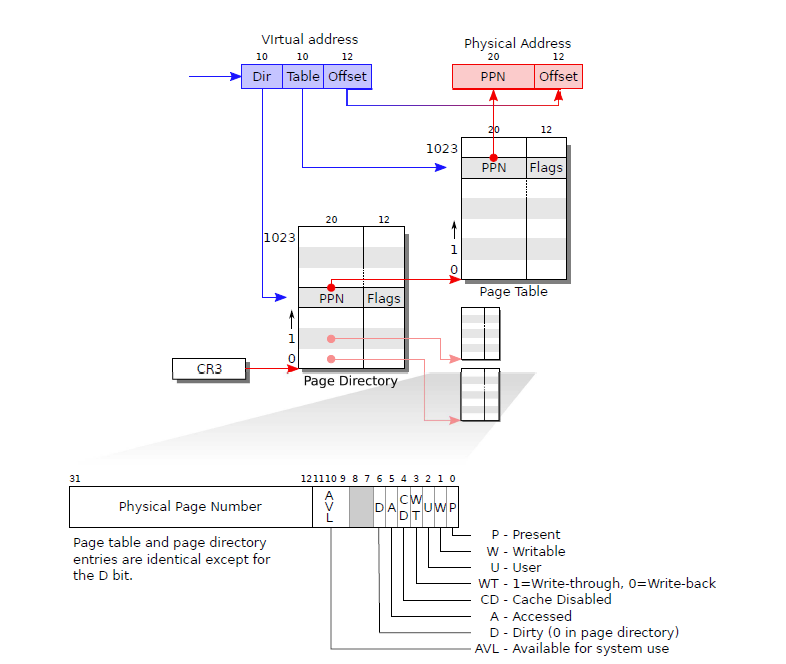
\includegraphics[width=0.8\textwidth]{img/pagemodel.PNG}
    \caption{xv6 page model}
    \label{fig:1}
\end{figure}

\textbf{./xv6 VM Layout/kernel/mmu.h}

\begin{ccode}
    // A linear address 'la' has a three-part structure as follows:
    //
    // +--------10------+-------10-------+---------12----------+
    // | Page Directory |   Page Table   | Offset within Page  |
    // |      Index     |      Index     |                     |
    // +----------------+----------------+---------------------+
    //  \--- PDX(la) --/ \--- PTX(la) --/
        
    // page directory index
    #define PDX(la)		(((uint)(la) >> PDXSHIFT) & 0x3FF)
        
    // page table index
    #define PTX(la)		(((uint)(la) >> PTXSHIFT) & 0x3FF)
        
    // construct linear address from indexes and offset
    #define PGADDR(d, t, o)	((uint)((d) << PDXSHIFT | (t) << PTXSHIFT | (o)))
\end{ccode}

每个页表项需要一些 flag 设置他们的属性,比如说 Writeable 表示可以写入,Present 表示这个页表已经被用到了。还可以指定被当成缓存时的各种策略

\textbf{./xv6 VM Layout/kernel/mmu.h}

\begin{ccode}
    // Page table/directory entry flags.
    #define PTE_P		0x001	// Present
    #define PTE_W		0x002	// Writeable
    #define PTE_U		0x004	// User
    #define PTE_PWT		0x008	// Write-Through
    #define PTE_PCD		0x010	// Cache-Disable
    #define PTE_A		0x020	// Accessed
    #define PTE_D		0x040	// Dirty
    #define PTE_PS		0x080	// Page Size
    #define PTE_MBZ		0x180	// Bits must be zero
\end{ccode}

\subsubsection{memory layout}

\begin{figure}[h]
    \centering
    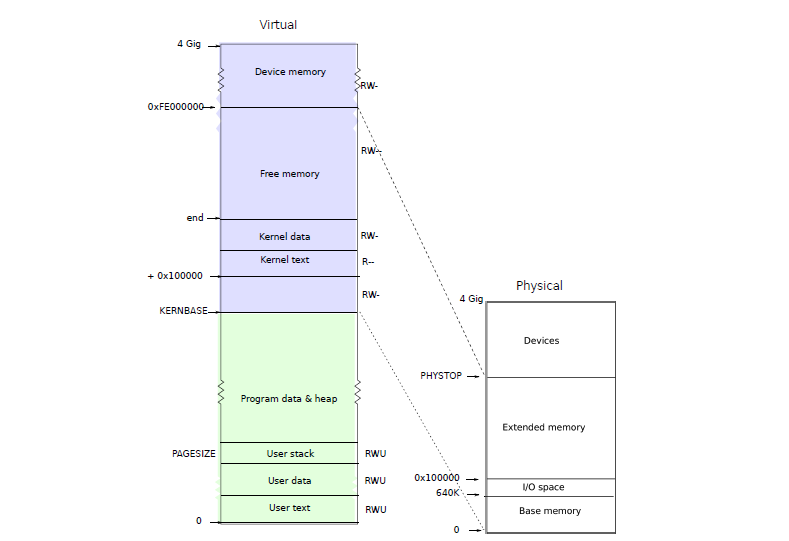
\includegraphics[width=0.8\textwidth]{img/memlayout.PNG}
    \caption{xv6 memory layout}
    \label{fig:2}
\end{figure}

用户内存从 0 开始一直到 KERNBASE。在 \textbf{./xv6 VM Layout/include/types.h} 中我们看到 NULL 被定义为 0。因此一个空指针会访问到 User text 部分,这部分的页表 flag 上有 \textbf{Present} 因此会被认为是一个合法的内存访问。现在我们希望把前两页空出来,这样当前两页将没有 `Present` flag,访问的时候 kernel 就会帮我们处理错误。

于是我们的任务主要就是:使得程序 (User text) 从 0x2000 开始存放,留出两页的空间,涉及到的更改有:

\begin{itemize}
    \item exec 执行程序会涉及到程序装载
    \item fork 复制出新的进程涉及到内存复制(程序装载)
    \item userinit 装载第一个用户程序需要特殊操作(涉及修改makefile)
    \item 修改相应的用户传入的地址的检查
\end{itemize}


\subsubsection{Code: exec}

exec 函数首先会检查 page table directory 是否设置,以及检查 elf header。不过我们的主要关注它如何分配内存

让我们先理解一些函数(无关紧要的细节已经被忽略)

\begin{itemize}
    \item \textbf{./xv6 VM Layout/kernel/kalloc.c kalloc} 该函数分配一个 4096 长度的物理内存空间
    \item \textbf{./xv6 VM Layout/kernel/vm.c walkpgdir} 返回页表地址
    \item \textbf{./xv6 Vm Layout/kernel/vm.c allocuvm} 为某个进程的页表分配新的空间,从 oldsz 增长到 newsz
    \item \textbf{./xv6 VM Layout/kernel/vm.c mappages} 该函数把会根据新分配的物理空间(4096长度)建立页表。也就是说会建立参数 la (虚拟地址) 到 pa (物理地址) 之间的映射。我们可以看到获取 `la` 的地址后会检查是否该地址已经被其他物理地址占用了(\textbf{panic("remap")}),否则就把 flag 加上 Present 一起添加。由之前的定义,相邻 page table directory 本来就有相邻的地址,如果这个 page table 满了自动就会应用到下一个 page table 中。(其实也可以看作是 $2^{20}$ 个连续页表)
\end{itemize}

回到 \textbf{exec} 为新程序分配内存的地方

\begin{ccode}
    sz = 0;
    for(i=0, off=elf.phoff; i<elf.phnum; i++, off+=sizeof(ph)){
        if(readi(ip, (char*)&ph, off, sizeof(ph)) != sizeof(ph))
        goto bad;
        if(ph.type != ELF_PROG_LOAD)
        continue;
        if(ph.memsz < ph.filesz)
        goto bad;
        if((sz = allocuvm(pgdir, sz, ph.va + ph.memsz)) == 0)
        goto bad;
        if(loaduvm(pgdir, (char*)ph.va, ip, ph.offset, ph.filesz) < 0)
        goto bad;
    }
    iunlockput(ip);
    ip = 0;
\end{ccode}



从 \textbf{sz=0} 开始然后再执行刚刚我们提到的 \textbf{allocuvm} 显然不是我们想要的结果,因为程序将从 0 开始装载而我们希望从 0x2000 开始,这里于是有两种思路

\begin{enumerate}
    \item 更改 allocuvm 当中的 mappages,使所有的内存空间都向后位移 0x2000
    \item 更改 exec,把程序的大小加大 0x2000
\end{enumerate}

事实上一开始我才用前者的策略但是稍加思考后我个人偏向后者,因为 \textbf{fork} 的时候会根据 \textbf{proc->sz} 复制内存地址。显然改变 \textbf{sz} 会使得事情简单很多,否则几乎要在每一个 \textbf{mappages} 的地方都留意是否要做更改

在进程的大小处做出更改

\begin{ccode}
    // sz = 0;
    sz = 0x2000;
\end{ccode}

看起来有疑问的地方

\begin{ccode}
    if((sz = allocuvm(pgdir, sz, ph.va + ph.memsz)) == 0)
    goto bad;
\end{ccode}

我们更改了初始 \textbf{sz} 的大小而没有动 \textbf{ph.va, ph.memsz},那么这里分配的内存会不会发生改变?其实不会,之后我们的更改会使得所有的用户程序 \textbf{sz} 都会增加保持一致性,使得这里留给程序的空间不会发生改变

用户程序的装在位置在 \textbf{./xv6 Vm Layout/user/makefile.mk} 需要被更改

\begin{bashcode}
    # location in memory where the program will be loaded
    USER_LDFLAGS += --section-start=.text=0x2000
\end{bashcode}

总之,在这一部分我们确保 \textbf{exec} 执行的程序从 \textbf{0x2000} 开始存放

\subsubsection{Code: fork}

\textbf{fork} 函数会创建新的进程,这个过程中会复制出新的页表,这里有一个地方也需要更改

\textbf{./xv6 VM Layout/kernel/vm.c copyuvm}

\begin{ccode}
    for(i = 0; i < sz; i += PGSIZE){
        if((pte = walkpgdir(pgdir, (void*)i, 0)) == 0)
        panic("copyuvm: pte should exist");
        if(!(*pte & PTE_P))
        panic("copyuvm: page not present");
        pa = PTE_ADDR(*pte);
        if((mem = kalloc()) == 0)
        goto bad;
        memmove(mem, (char*)pa, PGSIZE);
        if(mappages(d, (void*)i, PGSIZE, PADDR(mem), PTE_W|PTE_U) < 0)
        goto bad;
    }
\end{ccode}

在之前我们让 \textbf{sz} 增大了 \textbf{0x2000},因此这里复制地址看起来没什么问题,方便了许多。但是发现这里对每个在 \textbf{sz} 范围内的页表项都检查了必须要有 \textbf{Present} 标志,这就不是我们想要的了(前两页没有)。反正前两页我们不要,索性不复制了。这里就是第二个更改的地方

\begin{ccode}
    // for(i = 0; i < sz; i += PGSIZE){
    for (i=0x2000; i<sz; i += PGSIZE){
\end{ccode}

\subsubsection{Code: creating the first process}

第一个 user process 当然是我们的 shell 程序了,它可以在 \\
\textbf{./xv6 Vm Layout/user/init.c} 当中被找到

第一个 user process 既不是 fork 出来的也不是某个 user process 调用 exec 而出来的,它是手动设置的。它会先执行 initcode.S 中的程序(这也是一个程序所以当然也要从 0x2000开始),然后设置 trapframe 保留原始寄存器状态存放在 kernel stack 当中。从注释中我们发现,initCode 其实也是调用 exec 执行了 init 程序。我们让 userinit 的 eip 指向 initcode.S,设置进程状态为 RUNNABLE,然后交给 CPU 调度,准备让操作系统跑起来

于是我们要:

\begin{enumerate}
    \item 为了保留一致性我们需要更改这个手动设置的进程大小
    \item esp 位置需要更改为进程大小
    \item eip 需要指向 initcode.S 的位置也就是 0x2000
\end{enumerate}

\begin{ccode}
    p = allocproc();
    acquire(&ptable.lock);
    initproc = p;
    if((p->pgdir = setupkvm()) == 0)
    panic("userinit: out of memory?");
    inituvm(p->pgdir, _binary_initcode_start, (int)_binary_initcode_size);
    // p->sz = PGSIZE;
    p->sz = PGSIZE + 0x2000;
    memset(p->tf, 0, sizeof(*p->tf));
    p->tf->cs = (SEG_UCODE << 3) | DPL_USER;
    p->tf->ds = (SEG_UDATA << 3) | DPL_USER;
    p->tf->es = p->tf->ds;
    p->tf->ss = p->tf->ds;
    p->tf->eflags = FL_IF;
    // p->tf->esp = PGSIZE;
    p->tf->esp = p->sz;
    // p->tf->eip = 0;  // beginning of initcode.S
    p->tf->eip = 0x2000;
\end{ccode}

inituvm 装载了 init 程序,也需要更改开始位置

\begin{ccode}
    // Load the initcode into address 0 of pgdir.
    // sz must be less than a page.
    void
    inituvm(pde_t *pgdir, char *init, uint sz)
    {
    char *mem;
    
    if(sz >= PGSIZE)
        panic("inituvm: more than a page");
    mem = kalloc();
    memset(mem, 0, PGSIZE);
    // mappages(pgdir, 0, PGSIZE, PADDR(mem), PTE_W|PTE_U);
    mappages(pgdir, (void*)0x2000, PGSIZE, PADDR(mem), PTE_W|PTE_U);
    memmove(mem, init, sz);
    }
\end{ccode}

initcode 装载在哪里得找 makefile,第四个更改的地方:

\begin{bashcode}
    initcode: kernel/initcode.o
    $(LD) $(LDFLAGS) $(KERNEL_LDFLAGS) \
        --entry=start --section-start=.text=0x2000 \
        --output=kernel/initcode.out kernel/initcode.o
    $(OBJCOPY) -S -O binary kernel/initcode.out $@
\end{bashcode}

\subsubsection{one last step}

内核需要检查用户传递过来的指针是否合法。内核态什么时候需要用户态传递的信息?系统调用

系统调用从用户堆栈中获取参数。\textbf{argint(), argptr(), argstr() 会调用 fetchint(), fetchstr()} 根据地址获取内容。这里我们就要更新检查地址的内容,增加如果内容来自 $[0,0x2000)$ 就会报错

\begin{ccode}
    // Fetch the int at addr from process p.
    int
    fetchint(struct proc *p, uint addr, int *ip)
    {
        if (addr < 0x2000) return -1;
        if(addr >= p->sz || addr+4 > p->sz)
            return -1;
        *ip = *(int*)(addr);
        return 0;
    }

    // Fetch the nul-terminated string at addr from process p.
    // Doesn't actually copy the string - just sets *pp to point at it.
    // Returns length of string, not including nul.
    int
    fetchstr(struct proc *p, uint addr, char **pp)
    {
        char *s, *ep;
        if (addr < 0x2000) return -1;
        if(addr >= p->sz)
            return -1;
        *pp = (char*)addr;
        ep = (char*)p->sz;
        for(s = *pp; s < ep; s++)
            if(*s == 0)
            return s - *pp;
        return -1;
    }
\end{ccode}

\subsubsection{outcome}

别忘了 \textbf{执行 make clean} ! makefile 对于代码没有改变的文件(比如说 \textbf{init.c, initcode.S}) 不会重新编译。如果重新编译,他们还是会出现在 \textbf{0x0},然后就会困惑的发现程序会在 \textbf{schedule} 的时候出错 

经过一番修改后,我们运行之前的 \textbf{nulldereference}

\begin{textcode}
    xv6...
    lapicinit: 1 0xfee00000
    cpu1: starting
    cpu0: starting
    init: starting sh
    $ nulldereference
    pid 3 nulldereference: trap 14 err 4 on cpu 1 eip 0x2014 addr 0x0--kill proc
    $ 
\end{textcode}

当用户程序试图访问 \textbf{0x0} 时会发现那个地方的页表项没有 \textbf{Present} 标记,系统会通过 \textbf{trap} 退出